% (c) Gerard Baecker
\documentclass[fleqn,a4paper,12pt]{article}
\usepackage[german]{babel}
%\usepackage{amsmath}    % Mathematische Symbole
\usepackage{amssymb}     % Nochmehr mathematische Symbole
\usepackage{dsfont}      % Schriftsatz fuer Zahlenmengensymbole
%\usepackage{verbatim}   % erweiterte Verbatim-Umgebung
\usepackage{alltt}       % Quasi-Verbatim-Umgebung
\usepackage{fancyhdr}    % Eigene Kopfzeilen
\usepackage{graphicx}    % Zum Einbinden von Grafiken
% Einbinden einer eps-Grafik geht so: includegraphics{path}

% Seitenraender
\addtolength{\voffset}{-2cm}
\addtolength{\textheight}{0cm}
\addtolength{\hoffset}{0cm}
\addtolength{\textwidth}{2cm}
\addtolength{\headheight}{2cm} % fuer jeden Strichkode einen Zentimeter

% Skalierung der Grafiken
\setlength{\unitlength}{1cm}

\pagestyle{fancy}            % Eigene Kopfzeilen verwenden
\frenchspacing               % Kein Extrafreiraum nach Satzzeichen
\setlength{\parindent}{0pt}  % Neue Absaetze nicht einruecken
%\sloppy                     % Schlampige Absatzformatierung
\fussy                       % Penible Absatzformatierung
\linespread{1.5}             % Zeilenabstand

% Font fuer Code 39
\font\xlix=wlc39 scaled 1200
\newcommand\barcode[1]{{\xlix@#1@}}

% Name, Matrikelnummer, Barcode
\newcommand\student[2]{
  \mbox{\scriptsize
  \begin{tabular}{@{}l@{}r@{}}
    \multicolumn{2}{@{}r@{}}{\barcode{#2}}\\
    #1&#2\\
  \end{tabular}}}

% Kopfzeile
\lhead{
  \small
  \textsc{Grundlagen der Signalverarbeitung \\
    Sommersemester 2018 \\
    \"Ubung (\today)}
  \vfill}
\rhead{
  \begin{tabular}[b]{@{}rr@{}}
    \student{Linus Eckhard}{559369} &
    \student{Birk Leppich}{573744} \\
    \student{Adrian Dr{\"o}se}{572649}
  \end{tabular}}

\begin{document}
"Ubungsaufgabe 1: \newline

\begin{center}
\begin{tabular}{|p{10cm}|p{5cm}|}
	\hline \textbf{Prozess} & \textbf{Messbar?} \\
	\hline P"unktlichkeit der S-Bahn & Ja, man braucht den Fahrplan und eine Uhr. \\
	\hline Anzahl der Z"uge, um eine bestimmte Karte von einem Deck zu ziehen & Ja, man braucht einen Z"ahler. \\
	\hline Anzahl der Tage, bis man einen Bekannten ungeplant unterwegs trifft & Ja, man braucht einen Z"ahler. \\
	\hline
\end{tabular}
\end{center}

"Ubungsaufgabe 2: \newline

\begin{figure}[h]
\caption{Unbekannter Prozess im Laufe der Zeit}
\centering
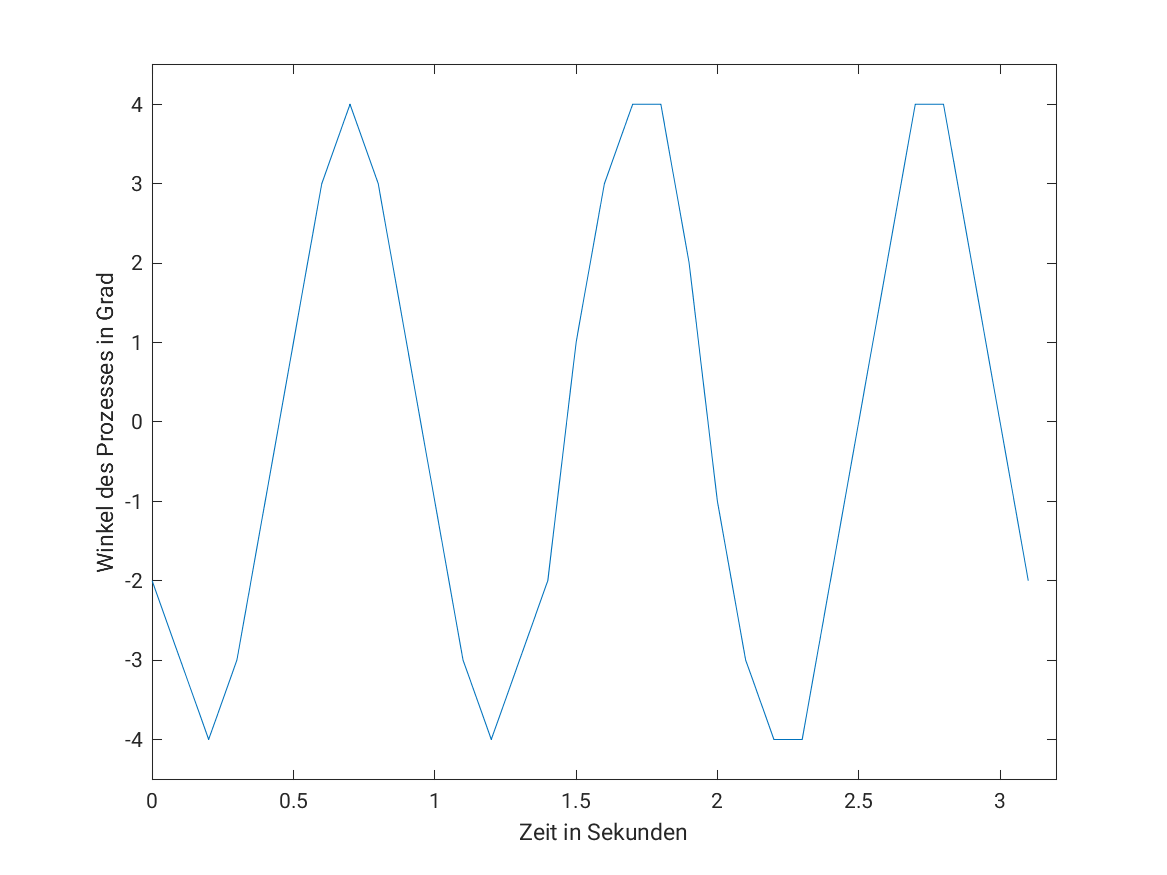
\includegraphics[width=1.0\textwidth]{unbekannterprozess}
\end{figure}

In Abbildung 1 ist der gemessene Winkel des unbekannten Prozesses im Verlauf der Zeit zu sehen. Anhand der Messwerte kann man erkennen, dass es sich hier um einen periodischen Prozess handelt, mit einer Periodenl"ange von ungef"ahr $1s$. Der Prozess ist somit nicht zuf"allig.

\end{document}
